\begin{center}
\textsc{\Large Laboratorio 13}~\\
{\large Vídeo Juegos, Físicas, Programación}~\\
\emph{Física en Vídeo Juegos, Simulaciones y Ragdolls}
\end{center}

\section{Pre-Laboratorio}
\todo[inline]{Por hacer.}

\section{Introducción}
Para agregar realismo, nuevas mecánicas o mayor calidad visual se introducen leyes físicas dentro del motor de juego, es mayormente usado en juegos tridimensionales \cite[p.~325]{jenkinscreatinggames}. Estas nuevos efectos se introducen en forma de simulaciones las cuales son aproximaciones de fenómenos reales utilizando valores discretos \cite{ian_gamephysics}. En el ambiente de un vídeo juegos una simulación completa y totalmente correcta podría causar complicaciones en las mecánicas de juego, progreso de la historia o hacer tediosas ciertas actividades.

\section{Simulaciones Físicas}
\setlength\intextsep{0pt}
\begin{wrapfigure}[7]{l}{0.4\linewidth}
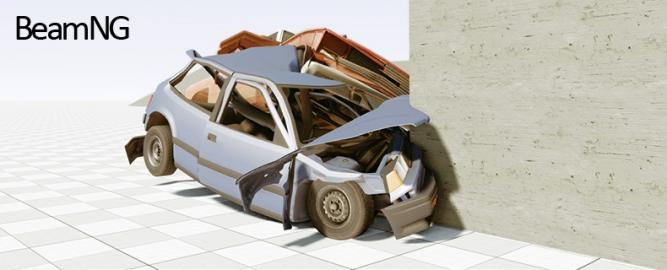
\includegraphics[width=\linewidth]{semana13/beamng_gamephysics.jpg}
\caption{BeamNG un video juego simulador de vehiculos que utiliza \emph{soft-body physics}.}
\label{fig:beamng}
\end{wrapfigure}
Hay dos clases centrales de simulaciones físicas, simulaciones de cuerpos rígidos (\emph{rigid-body physics}) y simulaciones de cuerpos blandos (\emph{soft-body physics}). En una simulación de cuerpos rígidos los objetos se agrupan entre categorías basadas en como deberían interaccionar, las simulaciones de cuerpos rígidos son menos intensas en cuanto a perdida de \emph{performance}. Las simulaciones de cuerpos blandos consisten en simular secciones individuales de cada objeto de tal forma que este se comporte de manera realista, usualmente utilizadas para simular objetos deformables como ropa o materiales destructibles \cite{ian_gamephysics}.
\section{Físicas \emph{Ragdoll}}
\setlength\intextsep{0pt}
\begin{wrapfigure}[10]{r}{0.4\linewidth}
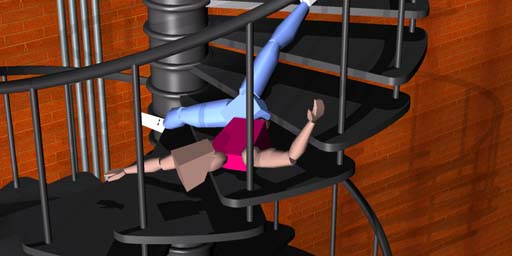
\includegraphics[width=\linewidth]{semana13/ragdoll.jpg}
\caption{Simulación de un personaje cayendo unas escalera, se utiliza un \emph{ragdoll}.}
\label{fig:ragdoll}
\end{wrapfigure}
Es una tecnica de simulacion que consiste en la animación procedimental de un personaje cuando este muere (u otro estado definido por el juego para causar \emph{ragdoll}, consiste en tratar a un objeto o personaje como una serie de objetos sólidos (huesos) conectados en distintos puntos formando un esqueleto. La simulación ocurre cuando el evento necesario para causar físicas \emph{ragdoll} sobre un objeto o personaje sucede, en los vídeo juegos esto pasa usualmente cuando el personaje muere \cite{eric_ragdoll}.

\section{Actividad}
\todo[inline]{Por hacer.}